\section{Spatial Discretization}
\label{sec:SpatialDiscretization}

\begin{defn}
  $R$ is called a \emph{square domain} if it can be written as
  $R=[\mathbf{x}_O,\mathbf{x}_E]$, where
  $\mathbf{x}_O,\mathbf{x}_E\in\mathbb{R}^D$.
\end{defn}
\begin{defn}
  $\Omega$ is called a \emph{regular domain} if it can be written as an
  union of finite disjoint square domains, i.e.
  \begin{equation}
    \Omega = \bigcup\limits_{k=1}^NR_k,
  \end{equation}
  where $R_k,\ k=1,\ldots,N$ are square domains.
\end{defn}

Denote the computational domain as $\Omega$ and  let $R$ be a regular domain
containing $\Omega$, we discretize $R$ into a
collection of square control volumes. Denote a control colume by a multi-index
$\mathbf{i}\in \mathbb{Z}^D$, then the region of cell $\mathbf{i}$ can be
represented by
\begin{equation}
  \label{eq:Ci}
  C_{\mathbf{i}}=\left[\mathbf{x}_O+\mathbf{i}h,\
    \mathbf{x}_O+(\mathbf{i}+\mathds{1}h\right],
\end{equation}
and the region of the higher face of cell $\mathbf{i}$ in dimension
$d$ by
\begin{equation}
  \label{eq:Fi}
  F_{\mathbf{i}+\frac{1}{2}\mathbf{e}^d}  :=
  \left[ \mathbf{\mathbf{x}_O} + \left(\mathbf{i}+\mathbf{e}^d \right)
    h, \mathbf{x}_O
    +\left(\mathbf{i}+\mathds{1}\right)h \right],
\end{equation}
where $\mathbf{x}_O\in\mathbb{R}^D$ is some fixed origin of the
coordinates, $h$ is the uniform grid size, $\mathds{1}\in\mathbb{Z}^D$
is the multi-index with all its components equal to one, and
$\mathbf{e}^d\in\mathbb{Z}^D$ is a multi-index with 1 as its $d$th
component and 0 otherwise.

For an irregular domain $\Omega$, we embed it into a discrete square
domain and  denote the corresponding cutting control volume and
control face as
\begin{equation}
  \mathcal{C}_{\mathbf{i}}:={C}_{\mathbf{i}}\cap \Omega,\quad
  \mathcal{F}_{\mathbf{i}+\frac{1}{2}\mathbf{e}^d} :=
  {F}_{\mathbf{i}+\frac{1}{2}\mathbf{e}^d}  \cap \Omega.
\end{equation}

We call $\mathcal{C}_{\mathbf{i}}$ an interior control volume if
$\mathcal{C}_{\mathbf{i}} = C_{\mathbf{i}}$, an exterior control volume
if $\mathcal{C}_{\mathbf{i}}=\emptyset$, a boundary control volume if
$\mathcal{C}_{\mathbf{i}}\neq C_{\mathbf{i}},\emptyset$. For a
boundary control volume, we denote its boundary as
\begin{equation}
  \label{eq:boundaryOfvolume}
  \mathcal{S}_{\mathbf{i}} := {C}_{\mathbf{i}}\cap\partial\Omega.
\end{equation}
There are the same classifications for control faces. Figure
\ref{fig:SpatialDiscretizationOfCD}  shows the spatial discretization
of two different computational domains:

\begin{figure}[htbp]
  \centering
  \subfigure[Sptial discretization of regular domain $R$]{
    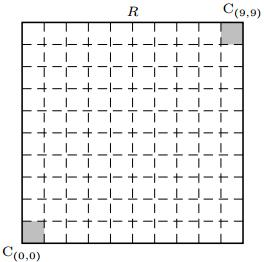
\includegraphics[width=0.3\textwidth]{regular.png}
  }
  \hspace{2cm}
  \subfigure[Spatial discretization $R(\Omega)$ of irregular domain (disc
  $\Omega$) embedded in the regular domain $R$, in which
  $\mathcal{C}_{(0,0)},\mathcal{C}_{(6,5)},\mathcal{C}_{(5,8)}$ is
  respectively an exterior, interior and boundary control volume.]{
    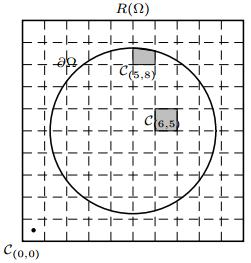
\includegraphics[width=0.3\textwidth]{irregular.png}}
  
  \caption{Sptial discretization of computational domain}
  \label{fig:SpatialDiscretizationOfCD}
\end{figure}

\begin{defn}
  Denote the average of a scalar function
  $\varphi:\mathbb{R}^D\rightarrow\mathbb{R}$ on a control volume
  $\mathcal{C}_{\mathbf{i}}$ as
  \begin{equation}
    \left<\varphi\right>_{\mathbf{i}} := \frac{1}{\Vert
      \mathcal{C}_{\mathbf{i}}\Vert}\int_{\mathcal{C}_{\mathbf{i}}}
    \varphi\  \mathrm{d}\mathbf{x}.
  \end{equation}
\end{defn}

\begin{defn}
  Denote the average of a scalar function
  $\varphi:\mathbb{R}^D\rightarrow\mathbb{R}$ on a control face
  $\mathcal{F}_{\mathbf{i}+\frac{1}{2}\mathbf{e}^d}$ as
  \begin{equation}
    \left<\varphi\right>_{\mathbf{i}+\frac{1}{2}\mathbf{e}^d} := \frac{1}{\Vert
      \mathcal{F}_{\mathbf{i}+\frac{1}{2}\mathbf{e}^d}\Vert}\int_{\mathcal{F}_{\mathbf{i}+\frac{1}{2}\mathbf{e}^d}}\varphi\
    \mathrm{d}\mathbf{x}.  
  \end{equation}
\end{defn}

\begin{defn}
  Denote the average of a scalar function
  $\varphi:\mathbb{R}^D\rightarrow\mathbb{R}$ on the boundary
  $\mathcal{S}_{\mathbf{i}}$ of a control volume as
  \begin{equation}
    \left[\varphi\right]_{\mathbf{i}} := \frac{1}{\Vert
      \mathcal{S}_{\mathbf{i}}\Vert}\int_{\mathcal{S}_{\mathbf{i}}}
    \varphi\  \mathrm{d}\mathbf{x}.
  \end{equation}
\end{defn}


There are three cases when discretizing operators:
\begin{enumerate}
\item For control volumes or faces in $\Omega$ which are far away
  from the boundary, we use standard finite volume stencils.
\item For control volumes or faces near the regular boundary, we
  fill the ghost cells with boundary conditions and then use standard
  finite volume formulas.
\item For control volumes or faces near the irregular boundary, we
  generate a poised lattice by poised lattice
  generating algorithm, then fit a complete
  multivariate polynomial with the poised lattice to obtain the
  discretized equation.
\end{enumerate}

\subsection{Standard finite difference formulas}
\label{sec:Standard}

In the regular domain, the discrete gradient, the discrete divergence and the dicrete
Laplacian are
\begin{eqnarray}
  \label{eq:G}
  \mathbf{G}_d\left<\phi\right>_{\mathbf{i}} &:=&
  \frac{1}{12h}\left(-\left<\phi\right>_{\mathbf{i}+2\mathbf{e}^d}
    +8\left<\phi\right>_{\mathbf{i}+\mathbf{e}^d}
    -8\left<\phi\right>_{\mathbf{i}-\mathbf{e}^d} 
  +\left<\phi\right>_{\mathbf{i}-2\mathbf{e}^d}\right) \\
  \label{eq:D}
  \mathbf{D}\left<\mathbf{u}\right>_{\mathbf{i}} &:=&
  \frac{1}{12h}\sum\limits_d \left( -\left<u_d\right>_{\mathbf{i}+2\mathbf{e}^d}
    +8\left<u_d\right>_{\mathbf{i}+\mathbf{e}^d}
    -8\left<u_d\right>_{\mathbf{i}-\mathbf{e}^d} 
                                                      +\left<u_d\right>_{\mathbf{i}-2\mathbf{e}^d}\right) \\
  \label{eq:L}
  \mathbf{L}\left<\phi\right>_{\mathbf{i}} &:=&
  \frac{1}{12h^2}\sum\limits_d\left(-\left<\phi\right>_{\mathbf{i}+2\mathbf{e}^d}
    +16\left<\phi\right>_{\mathbf{i}+\mathbf{e}^d} - 30\left<\phi\right>_{\mathbf{i}} 
    +16\left<\phi\right>_{\mathbf{i}-\mathbf{e}^d} 
  -\left<\phi\right>_{\mathbf{i}-2\mathbf{e}^d}\right) \\
\end{eqnarray}

The discrete divergence also acts on tensor averages
\begin{equation}
  \label{eq:Duu}
  \mathbf{D}\left<\mathbf{uu}\right>_{\mathbf{i}} :=
  \frac{1}{h}\sum\limits_d\left(
    \mathbf{F}\left<u_d,\mathbf{u}\right>_{\mathbf{i}+\frac{1}{2}\mathbf{e}^d}
    -
    \mathbf{F}\left<u_d,\mathbf{u}\right>_{\mathbf{i}-\frac{1}{2}\mathbf{e}^d}  \right),
\end{equation}
where the average of the product of two scalars over a cell face is
\begin{equation}
  \label{eq:ProductOf2scalar}
  \mathbf{F}\left<\phi,\psi\right>_{\mathbf{i}+\frac{1}{2}\mathbf{e}^d}
  :=
  \left<\phi\right>_{\mathbf{i}+\frac{1}{2}\mathbf{e}^d}
  \left<\psi\right>_{\mathbf{i}+\frac{1}{2}\mathbf{e}^d}+
  \frac{h^2}{12}\sum\limits_{d'\neq
    d}\left(\mathbf{G}^{\perp}_{d'}\phi\right)_{\mathbf{i}+\frac{1}{2}\mathbf{e}^d}
  \left(\mathbf{G}^{\perp}_{d'}\psi\right)_{\mathbf{i}+\frac{1}{2}\mathbf{e}^d},
\end{equation}
and $\mathbf{G}^{\perp}_{d'}$ is the discrete gradient in the
transverse directions
\begin{equation}
  \label{eq:TransverseG}
  \left(\mathbf{G}^{\perp}_{d'}\phi\right)_{\mathbf{i}+\frac{1}{2}\mathbf{e}^d}
  :=
  \frac{1}{2h}\left(\left<\phi\right>_{\mathbf{i}+\frac{1}{2}\mathbf{e}^d+\mathbf{e}^{d'}}-
  \left<\phi\right>_{\mathbf{i}+\frac{1}{2}\mathbf{e}^d-\mathbf{e}^{d'}}
 \right)
\end{equation}

$\mathbf{G}\left<\phi\right>,\ \mathbf{D}\left<\mathbf{u}\right>,\
\mathbf{L}\left<\mathbf{u}\right>$ and 
$\mathbf{D}\left<\mathbf{uu}\right>$ approximate the cell average of a
gradient, velocity divergence, Laplacian, and convection,
respectively. These discrete operators are fomally fourth-order
accurate in approximating their continuous
counterparts.\cite{zhang_fourth-order_2014}\cite{zhang_fourth-order_2012}

\subsection{Ghost Cell}
\label{sec:GhostCell}

Following \cite{zhang_fourth-order_2014}, two layers of ghost cells
are used to enforce boundary  
conditions.  For nonperiodic boundaries, the values of ghost cells are
obtained by extrapolating those of the interior cells, with the
boundary conditions incorporated in the extrapolation formulas. For
example, homogeneous Dirichlet boundary conditions for a scalar $\psi$
are fulfilled by filling the ghost cells with the following
fifth-order formulas:
\begin{equation}
  \label{eq:GhostedDiri}
  \begin{aligned}
    \left<\psi\right>_{\mathbf{i}+\mathbf{e}^d} = \frac{1}{12}\left(
      -77\left<\psi\right>_{\mathbf{i}} +
      43\left<\psi\right>_{\mathbf{i}-\mathbf{e}^d} -
      17\left<\psi\right>_{\mathbf{i}-2\mathbf{e}^d} +
      3\left<\psi\right>_{\mathbf{i}-3\mathbf{e}^d}\right) + O(h^5), \\
    \left<\psi\right>_{\mathbf{i}+2\mathbf{e}^d} = \frac{1}{12}\left(
      -505\left<\psi\right>_{\mathbf{i}} +
      335\left<\psi\right>_{\mathbf{i}-\mathbf{e}^d} -
      145\left<\psi\right>_{\mathbf{i}-2\mathbf{e}^d} +
      27\left<\psi\right>_{\mathbf{i}-3\mathbf{e}^d}\right) + O(h^5),
  \end{aligned}
\end{equation}
Neumann boundary conditions are fulfilled by
\begin{equation}
  \label{eq:GhostedNeumann}
  \begin{aligned}
    \left<\psi\right>_{\mathbf{i}+\mathbf{e}^d} = \frac{1}{10}\left(
      5\left<\psi\right>_{\mathbf{i}} +
      9\left<\psi\right>_{\mathbf{i}-\mathbf{e}^d} -
      5\left<\psi\right>_{\mathbf{i}-2\mathbf{e}^d} +
      \left<\psi\right>_{\mathbf{i}-3\mathbf{e}^d}\right) +
    \frac{6}{5}h\left<\pdfFrac{\psi}{n}\right>_{\mathbf{i}+\frac{1}{2}\mathbf{e}^d} + O(h^5), \\
    \left<\psi\right>_{\mathbf{i}+2\mathbf{e}^d} = \frac{1}{10}\left(
      -75\left<\psi\right>_{\mathbf{i}} +
      145\left<\psi\right>_{\mathbf{i}-\mathbf{e}^d} -
      75\left<\psi\right>_{\mathbf{i}-2\mathbf{e}^d} +
      15\left<\psi\right>_{\mathbf{i}-3\mathbf{e}^d}\right) +
    6h\left<\pdfFrac{\psi}{n}\right>_{\mathbf{i}+\frac{1}{2}\mathbf{e}^d}
    + O(h^5),
  \end{aligned}
\end{equation}
where
$\left<\pdfFrac{\psi}{n}\right>_{\mathbf{i}+\frac{1}{2}\mathbf{e}^d} $
is the Neumann condition for $\psi$. 

\subsection{PLG}
\label{sec:PLG}

For the control volumes and faces near the irregular boundary, where
we can not use standard difference formulas, our idea is:
\begin{enumerate}
\item Clarify the control volume $\mathcal{C}_{\mathbf{i}}$ (or
  control face $\mathcal{F}_{\mathbf{i}+\frac{1}{2}\mathbf{e}^d}$)
  where differential operator $\mathcal{L}$ is to be discretized, the order of
  spatial discretization $p$, and the average of differential
  operator on control volumes 
  $\left\{\left<\varphi\right>_{\mj}:\mj\in\mathbb{Z}^D\right\}$ (or
  on control faces
  $\left\{\left<\varphi\right>_{\mj}:\mj\in\mathbb{Z}^D+\frac{1}{2}\me^d\right\}$
  ).
\item As shown in Figure \ref{fig:PLGfigure}, we calculate finite volume stencil of
  $\left<\mathcal{L}\varphi\right>_{\mi}$ with poised lattice
  generating algorithm, denote it as
  \begin{equation}
    \label{eq:Stencil}
    \mathcal{X}(\mi) =
    \{\mathcal{C}_{\mj_1},\cdots,\mathcal{C}_{\mj_N}\} \cup
    \{\mathcal{S}_{\mj_{N+1}},\cdots,\mathcal{S}_{\mj_{N+N'}}\}
  \end{equation}
  where $N=\dim\Pi_n^D$, $n=p+q-1$ is the order of stencil, $q$ is the
  order of differential operator, $N'$ is the number of boundary
  terms.

   \begin{figure}[htbp]
  \centering
  \subfigure[A poised lattice in $\Pi^2_4$ at the hollow dot]{
    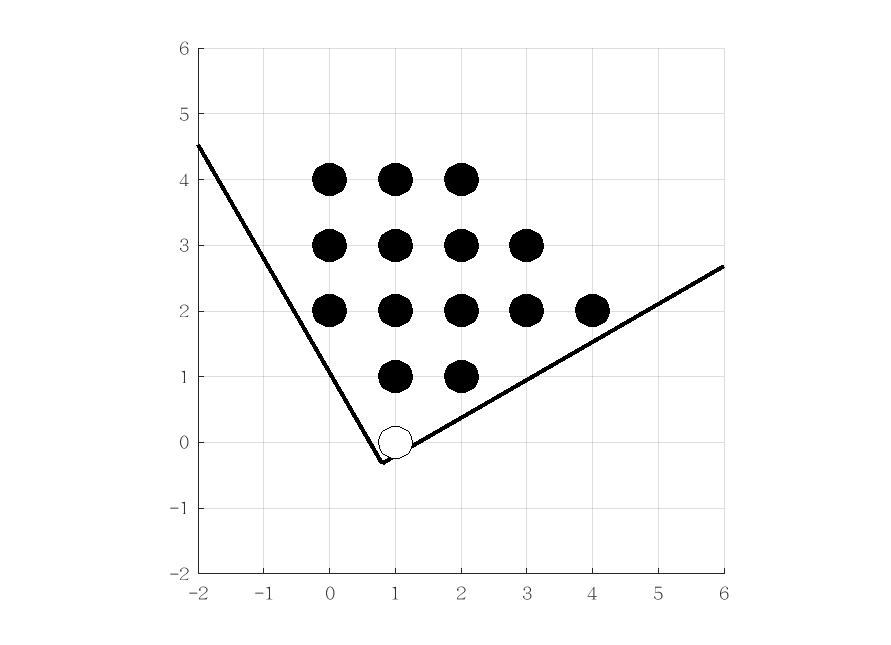
\includegraphics[width=0.35\textwidth]{S-2-4-bx.png}
  }
  \hspace{2cm}
  \subfigure[A poised lattice in $\Pi^3_3$ at the hollow dot]{
    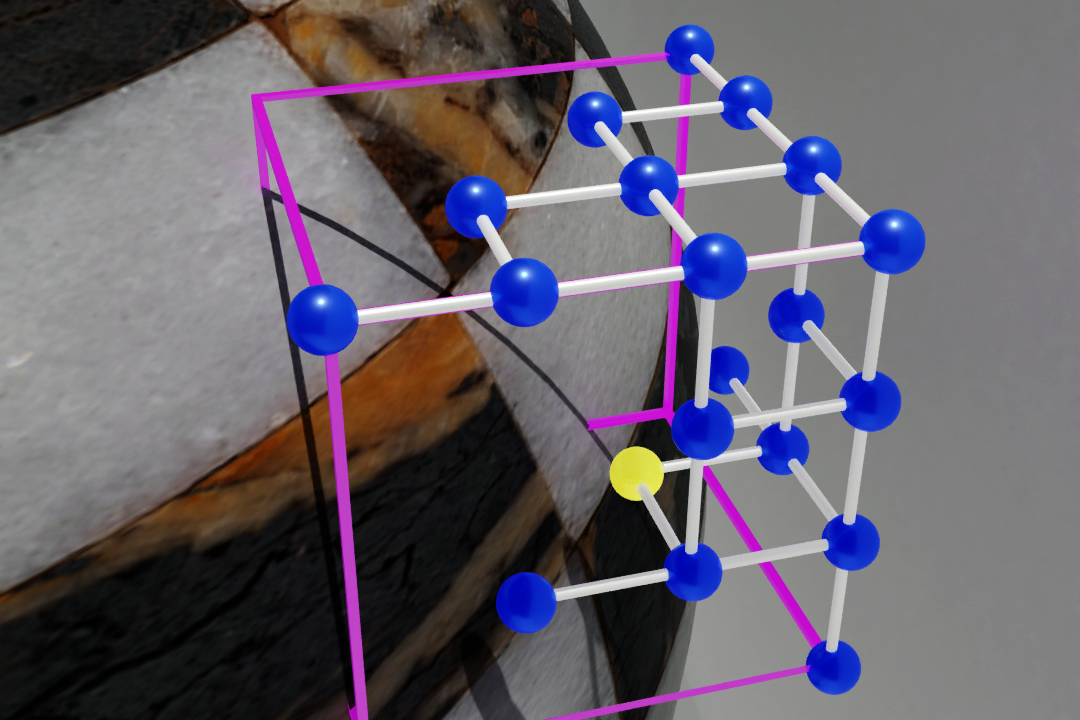
\includegraphics[width=0.35\textwidth]{S-3-3-cv.png}}
  
  \caption{For a given starting point, we choose a set of nodes to fit
  a high-order, multi-variate, complete polynomial, which facilitates
  the discretization of spatial operators and the enforcement of
  boundary conditions.}
  \label{fig:PLGfigure}
\end{figure}

\item Fit a complte multivariate polynomial with the finite volume
  stencil $\mathcal{X}(\mi)$:
  \begin{equation}
    \label{eq:FittingPoly}
    p(\mx)=\sum\limits_{j=1}^N \alpha_j\phi_j(\mx)\in\Pi_n^D,
  \end{equation}
  where $\left\{\phi_j\right\}_{j=1}^N$ is a basis of $\Pi_n^D$,
  coefficient $\mathbf{\alpha} = [\alpha_1,\cdots,\alpha_n]^T$ is the
  solution of weighted least squares problem
  \begin{equation}
    \label{eq:WeightedLSP}
    \min_{\alpha}\sum_{k=1}^N\omega_k\left|\left<p\right>_{\mj_k} -
      \varphi_k\right|^2 +
    \sum_{k=N+1}^{N=N'}\omega_k\left|\left[\mathcal{N}p\right]_{\mj_k} -
    \varphi_k\right|^2,
  \end{equation}
  where weight $\omega_k$ depends on the relative position of
  $\mathcal{C}_{\mj_k}$ and $\mathcal{C}_{\mi}$.
\item Finally discretize the differential operator with fitted
  polynomial \eqref{eq:FittingPoly}:
  \begin{equation}
    \label{eq:DiscreteOp}
    \left<\mathcal{L}\varphi\right>_{\mi} =
    \left<\mathcal{L}p\right>_{\mi}  + O(h^p) =
    \sum_{k=1}^N\beta_k\left<\varphi\right>_{\mj_k}+
    \sum_{k=N+1}^{N+N'}\beta_k\left[\mathcal{N}\varphi\right]_{\mj_k} + O(h^p).
  \end{equation}
\end{enumerate}

Now we obtain the fourth-order (spatial) semi-discrete formulas of
GePuP \eqref{eq:GePuP} for incompressible Navier-Stokes equations.

\begin{subequations}
  \label{eq:SemiGePuP}
  \begin{eqnarray}
  &\frac{\mathrm{d}\left<\mathbf{w}\right>}{\mathrm{d}t}=
  \left<\mathbf{g}\right>-\mathbf{D}\left<\mathbf{uu}\right>
    -\mathbf{G}\left<q\right> +
    \nu\mathbf{L}\left<\mathbf{w}\right> \mbox{ in } \Omega,
    \label{eq:SemiGePuPa}\\
  &\left[\mathbf{w}\right]=0 \mbox{ on }\partial \Omega, \\
  &\left<\mathbf{u}\right>=\mathbb{P}\left<\mathbf{w}\right>\mbox{ in
    } \Omega, \\
  &\left[\mathbf{u\cdot n}\right]=0\mbox{ on }\partial \Omega,\\
  &\mathbf{L}\left<q\right> =
  \mathbf{D}(\left<\mathbf{g}\right>-\mathbf{D}\left<\mathbf{uu}\right>)
    \mbox{ in }\Omega,\\
  &\left[\mathbf{n}\cdot\nabla q\right]=
  \left[\mathbf{n}\cdot\mathbf{g}\right]+\nu\left[(\mathbf{n}\cdot\mathbf{L})\mathbf{u}\right]-\nu\left[(\mathbf{n\cdot
    G})\mathbf{D}\mathbf{u}\right]\mbox{
  on } \partial \Omega.
\end{eqnarray}
\end{subequations}
with the initial conditions
\begin{subequations}
  \label{eq:SemiGePuPInitialCond}
  \begin{eqnarray}
    &\left<\mathbf{u}\right>(t_0)=\left<\mathbf{w}\right>(t_0),\\
    &\left[\mw\right]=\mathbf{0}.
  \end{eqnarray}
\end{subequations}



%%% Local Variables:
%%% mode: latex
%%% TeX-master: "MGPreconditioner_MathDoc"
%%% End:
